%standard 14.1

%start_of_questions


%new_question
%%%%%%%%%%%%%%%%%%%%%
	% Problem 1
	% Difficulty: 1
%%%%%%%%%%%%%%%%%%%%%
	\item 
		Write 100 integers created randomly into a file named \textit{QuizInts.txt}. 
		The numbers should be between 50 and 200 (inclusively). 
		Each number should be on a new line.\\
		Hint: Your code will likely use the following two lines of code somewhere in your program.\\
			\tab import random.\\
			\tab random.randint(50,200)

%new_question
%%%%%%%%%%%%%%%%%%%%%
	% Problem 2
	% Difficulty: 1
%%%%%%%%%%%%%%%%%%%%%			
	\item 
		Write a Python program that will open a file named \textit{thisFile.txt} and write every 
		other line into the file
		\textit{thatFile.txt}

%new_question
%%%%%%%%%%%%%%%%%%%%%
	% Problem 3
	% Difficulty: 1
%%%%%%%%%%%%%%%%%%%%%
	\item
		Create a file named \textit{MyName.txt}, and write your name to it (your actual name).	 
		Then read the file and print the letters of your name one at a time where each letter is on a new line.
		\begin{figure}[ht]
			\centering
			\begin{minipage}[b]{.4\textwidth}
				\centering
				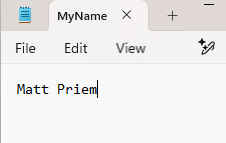
\includegraphics[scale=1]{imgs/nameFile.png}
				\caption{This is the file.}	
			\end{minipage}
			\hspace*{2em}
			\begin{minipage}[b]{.4\textwidth}
				\centering
				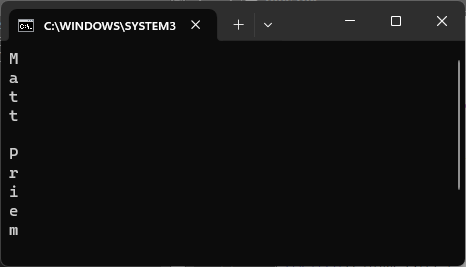
\includegraphics[width=1\textwidth]{imgs/nameOutput.png}
				\caption{This is the output.}
			\end{minipage}
		\end{figure}


%new_question
%%%%%%%%%%%%%%%%%%%%%
	% Problem 4
	% Difficulty: 1
%%%%%%%%%%%%%%%%%%%%%		
	\item
		Assume you are working on a file named \textit{MyCode.py} and there is a file \textit{MyWords.txt} in the same 
		working directory (same folder). The \textit{MyWords.txt} file contains exactly 20 words all written on separate
		lines. Read the file, and then write the words to a new file in four lines of five words.



%new_question
%%%%%%%%%%%%%%%%%%%%%
	% Problem 6
	% Difficulty: 1
%%%%%%%%%%%%%%%%%%%%%
	\item
		Assume you have a text file called \textit{aMorePerfectUnion.txt} that contains a transcript 
		of Barack Obama's March $18^{th}$, 2008 speech \textit{A More Perfect Union}. Create a 
		dictionary consisting each word and the amount of times that word appears in the speech. 
		Print the dictionary.

%end_of_questions
%make sure to leave at least one blank line below

